\documentclass[12pt]{article}
\usepackage{graphicx, epstopdf}

\begin{document}
\title{Summary report of rejection email analysis}
\author{Davide Chiuchiu}

\maketitle

\section{Scope}
This document contains my findings on the corpus of emails that I received during my job search. The email database contains 
\begin{itemize}
	\item the emails that confirmed the application submission
	\item the emails where companies showed interest in pursuing further my candidacy
	\item the emails where companies rejected my candidacy.
\end{itemize}

\section{Companies tends to be very concise when they interact with applicants.}
The first thing I notice from my analysis is that companies tends to be very concise when they interact with applicants. Overall the email I have received during my job search are quite short (see Figure \ref{fig:email_lengths}). Their majority s has less than 10 sentences, with 4-7 sentences as the most common length. 

\begin{figure}
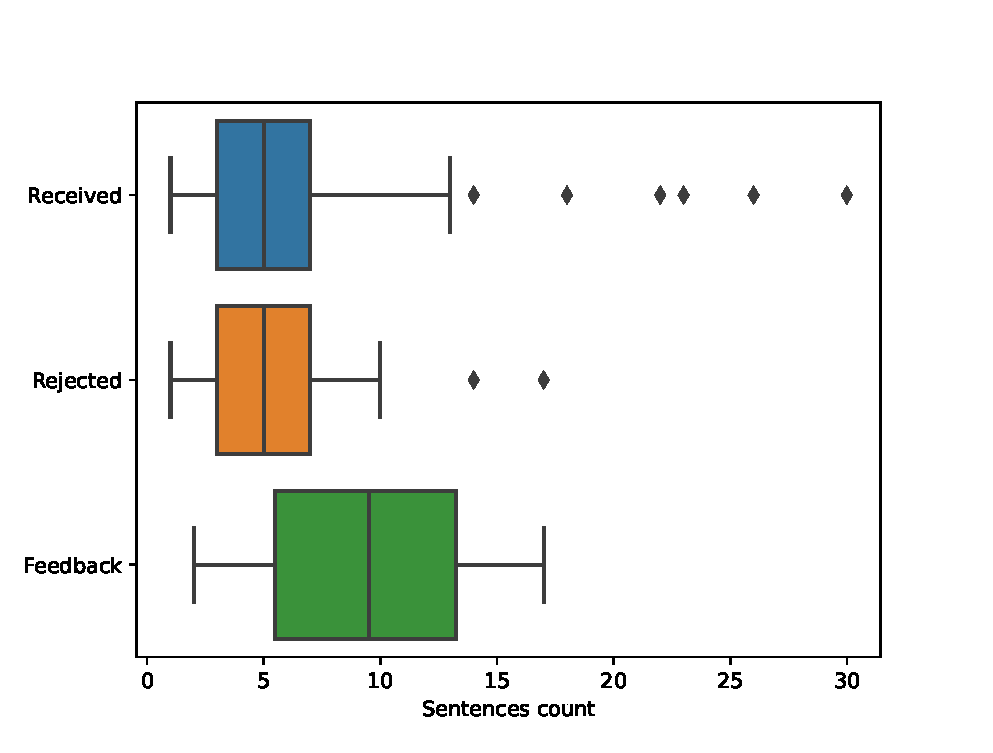
\includegraphics[width = \linewidth]{message_length_distribution.eps}
\caption{Companies tends to be very concise when they interact with applicants. Emails from companies rarely have more than 10 sentences. \label{fig:email_lengths}}
\end{figure}

\end{document}